\documentclass[journal,12pt,twocolumn]{IEEEtran}
\usepackage{cite}
\usepackage{amsmath,amssymb,amsfonts,amsthm}
\usepackage{algorithmic}
\usepackage{graphicx}
\usepackage{textcomp}
\usepackage{xcolor}
\usepackage{txfonts}
\usepackage{listings}
\usepackage{enumitem}
\usepackage{mathtools}
\usepackage{gensymb}
\usepackage{comment}
\usepackage[breaklinks=true]{hyperref}
\usepackage{tkz-euclide} 
\usepackage{textgreek}                       
\usepackage{circuitikz}
\usepackage{pgfplots}                            
\usepackage[latin1]{inputenc}                                
\usepackage{color}                                            
\usepackage{array}                                            
\usepackage{longtable}                                       
\usepackage{calc}                                             
\usepackage{multirow}                                         
\usepackage{hhline}                                           
\usepackage{ifthen}                                           
\usepackage{lscape}

\newtheorem{theorem}{Theorem}[section]
\newtheorem{problem}{Problem}
\newtheorem{proposition}{Proposition}[section]
\newtheorem{lemma}{Lemma}[section]
\newtheorem{corollary}[theorem]{Corollary}
\newtheorem{example}{Example}[section]
\newtheorem{definition}[problem]{Definition}
\newcommand{\BEQA}{\begin{eqnarray}}
\newcommand{\EEQA}{\end{eqnarray}}
\newcommand{\define}{\stackrel{\triangle}{=}}
\theoremstyle{remark}
\newtheorem{rem}{Remark}

\begin{document}

\bibliographystyle{IEEEtran}
\vspace{3cm}

\title{NCERT 11.9.2  Q7}
\author{EE23BTECH11204- Ashley Ann Benoy$^{*}$% <-this % stops a space
}
\maketitle
\newpage
\bigskip

\renewcommand{\thefigure}{\theenumi}
\renewcommand{\thetable}{\theenumi}

\bibliographystyle{IEEEtran}
\textbf{Question:
Find the sum of n terms of the A.P. whose kth term is 5k + 1. }\\


\textbf{
\begin{table}[htbp]
\centering
\caption{Given Data}
\label{tab:data}
\begin{tabular}{|c|c|c|}
\hline
\textbf{Symbol} & \textbf{Value} & \textbf{Parameter} \\
\hline
\(x_0\) & \(1 \) & First Term \\
\hline
\(x_k\) & \(5k + 1 \) & kth Term \\
\hline
\(d\) & \(5 \) & Common Difference \\
\hline
\(S_n\) & \(?\) & Sum of \(N\) terms \\
\hline
\end{tabular}
\end{table}
}

Given:
\[
\text{kth term of AP: } a_k = 5k + 1
\]

Sequence Representation:
The given arithmetic progression (AP) can be represented as:
\begin{align}
x(n) = (5n + 1)u(n)
\end{align}
where \( u(n) \) is the unit step function.

Z-transform:
Apply the Z-transform to \( x(n) \):
\begin{align}
x(z) = \frac{5 + z^{-1}}{(1 - z^{-1})^2}
\end{align}

Region of Convergence or R.O.C :
\begin{align}
     \lvert z \rvert > 1
\end{align}

Sum of First \( n+1 \) Terms:
Express the sum of the first \( n+1 \) terms (\( y(n) \)) in terms of \( x(n) \) using the convolution:
\begin{align}
y(n) = x(n) * u(n)
\end{align}

Inverse Z-transform:
Apply the Z-transform on both sides to get \( Y(z) = X(z)U(z) \), where \( U(z) \) is the Z-transform of the unit step function.
\begin{align}
Y(z) = \frac{5 + z^{-1}}{(1 - z^{-1})^2}
\end{align}

Contour Integration for Inverse Z-transform:
Use contour integration to find the inverse Z-transform (\( y(n) \)):
\begin{align}
y(n) = \frac{1}{2\pi j} \oint_C Y(z)z^{n-1} \,dz
\end{align}

Residue Calculations:
Calculate the residues \( R_1 \) and \( R_2 \) at the poles of the Z-transform.
\begin{align}
R_1 = 5(n+1) 
\end{align}
\begin{align}
R_2 = -n
\end{align}
\begin{align}
S_n = r_1 + r_2 = 4n + 5
\end{align}

\begin{figure}[h]
  \centering
  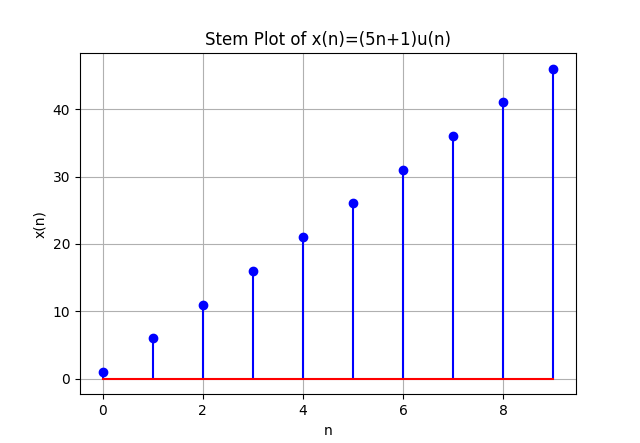
\includegraphics[width=0.6\textwidth]{figs/stem.png}
 
  \label{fig:Stem_Plot}
\end{figure}
\end{document}

